\chapter{Implementation}
This chapter covers how each stage was implemented, including code snippets, diagrams of how each component is linked and decisions that were made.
\section{CartPole}
CartPole is a pre-built environment from the Gym library, therefore, it just has to be imported using:
\begin{center}
    gym.make('CartPole-v1')
\end{center}

In this experiment version 1 was prefered over version 0 as it provides more timesteps, setting the limit to 500 timesteps per episode.

There are three main parts in stage 1:
\begin{figure}[H]
    \centering
    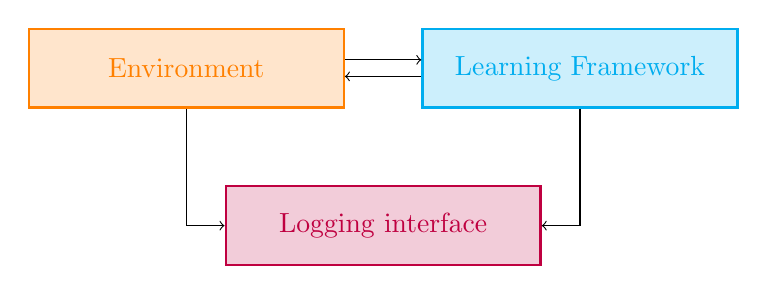
\begin{tikzpicture}
        \node[rectangle, 
        draw, 
        thick,
        minimum width = 4cm,
        minimum height = 1cm,
        color=orange,
        fill=orange!20,
        ] (A) at (0,0)  {Environment};
        \node[rectangle, 
        draw, 
        thick,
        minimum width = 4cm,
        minimum height = 1cm,
        color=cyan,
        fill=cyan!20,
        ] (B) at (5,0)  {Learning Framework};
        \node[rectangle, 
        draw, 
        thick,
        minimum width = 4cm,
        minimum height = 1cm,
        color=purple,
        fill=purple!20,
        ] (C) at (2.5,-2)  {Logging interface};

        \draw[->] ([yshift=3]A.east) -- ([yshift=3]B.west);
        \draw[<-] ([yshift=-3]A.east) -- ([yshift=-3]B.west);
        \draw[->] (B.south) |- (C.east);
        \draw[->] (A.south) |- (C.west);

        
    \end{tikzpicture}
\end{figure}

Each of these should interact for a successful implementation of the first stage.
After the environment is imported, the learning framework is imported, this is a framework used to train the agent.
Two main implementations were explored in this stage, Keras-rl and a manual implementation of the Keras API.

    \subsection*{Keras-rl}
    To implement keras-rl\cite{kerasrl2} in the specific hardware used in this project, it was required to be installed from source inside a miniforge environment.
    To be able to set up the model used by Keras-rl, TensorFlow was required. Once again, the hardware required a custom installation, the instructions can be found on the manufactures website \cite{apple-tf}.

    As the requirements were met, the next step is to setup a model, this was setup using keras, imported from TensorFlow.
\begin{figure}[H]
    \centering
    \includegraphics[width=1\textwidth]{cartpole_neural_network.eps}
    \caption{Visual representation of the neural network used to solve the CartPole Environment. }
    \label{fig:cartpole_neural_network}
\end{figure}
An implementation of the neural network used for the CartPole environment, using the structure demonstrated above is shown in the code snippet below.

\lstset{language=Python}
\lstset{frame=lines}
\lstset{caption={Setting up the model in the CartPole environment}}
\lstset{label={lst:code_direct}}
\lstset{basicstyle=\footnotesize}
\begin{lstlisting}
from tensorflow.keras.models import Sequential
from tensorflow.keras.layers import Dense, Input

states = env.observation_space.shape
actions = env.action_space.n

def build_model(states, actions):
model = Sequential() 
model.add(Input(states))
model.add(Dense(12, activation='relu', input_shape=(1,4)))
model.add(Dense(12, activation='relu'))
model.add(Dense(actions, activation='linear'))
return model

model = build_model(states, actions)
model.build(states)
\end{lstlisting}
    
    The code displayed above is used to import the required packages for the model, proceeded by a function where the model is defined. Here, we can see that the model receives the inputs and it connect to a fully-connected (Dense) layer with 12 neurons and relu activation function,
    this layer is followed by another fully connected layer with 12 neurons and relu activation function.
    
    The next step in setting up the learning framework is to define the agent. To do this, Keras-rl needs to be imported.
    
\lstset{language=Python}
\lstset{frame=lines}
\lstset{caption={Setting up the learning agent}}
\lstset{basicstyle=\footnotesize}
\begin{lstlisting}
from rl.agents import DQNAgent
from rl.policy import EpsGreedyQPolicy
from rl.memory import SequentialMemory          
from tensorflow.keras.optimizers import Adam

def build_agent(model, actions):
    policy = EpsGreedyQPolicy(eps=.3)
    memory = SequentialMemory(limit=50000, window_length=1)
    dqn = DQNAgent(model=model, memory=memory, 
    policy=policy, nb_actions=actions, 
    nb_steps_warmup=100, target_model_update=1e-2)
    return dqn

dqn = build_agent(model, actions)
dqn.compile(Adam(learning_rate=0.01), metrics=["mae"])

dqn.fit(env, nb_steps=50000)
\end{lstlisting}

In the code above, the agent, exploration policy and memory are imported from the Keras-rl library and the Adam optimizer is imported from Keras.

The $build\_agent$ function is used to set the DQNAgent, the exploration policy is initiated and $\epsilon$ value is set to 0.3.
The memory, replay buffer, is initiated using the SequentialMemory class from Keras-rl, the memory length is set to 50000 samples and the window length is set to the number of samples at each time, in this case 1.
The agent is then compiled using the Adam optimizer, where the learning rate is set to the optimal value of 0.01, here the metric use is also set to the mean absolute error.
The DQNAgent is now initiated using the model, policy and memory previously defined, along with this, the number of actions is passed as a parameter, the number of warmup steps used to avoid oscillating parameters and the target model update is set to 1e-2, this indicates how the target model is updated based on the model being trained.

The last line is used to train the agent, the environment is passed as a parameter and the number of steps is set to 50000.

\subsection*{Manual Agent implementation}
During the CartPole stage, another implementation was tested against Keras-rl, this was a manual implementation of the agent.
An agent can be split into multiple parts:
\begin{itemize}
    \item Replay buffer
    \item Action selection
    \item Target-q model update
    \item Training
\end{itemize}

The \textbf{replay buffer} is used to store the following sets of data (state, action, reward, state', done), than this is sampled in batches, this batches are used to train the neural network, the replay buffer is implemented to allow learning multiple times from the same actions and it also helps to break correlations.
\lstset{language=Python}
\lstset{frame=lines}
\lstset{caption={The following function is used to store the sets of data in the replay buffer}}
\lstset{basicstyle=\footnotesize}
\begin{lstlisting}
def remember(self, state, action, reward, next_state, done):
    item = (state, action, reward, next_state, done)
    self.memory.append(item)
\end{lstlisting}


\lstset{language=Python}
\lstset{frame=lines}
\lstset{caption={The following function is used to replay actions from the buffer and train the neural network using this}}
\lstset{basicstyle=\footnotesize}
\begin{lstlisting}
def replay(self, batch_size):
    batch = random.sample(self.memory, batch_size)
    state_batch, target_batch = [], []

    for state, action, reward, next_state, done in batch:
        target = self.get_target_q_value(state)
        if done:
            target[0][action] = reward
        else:
            Q_future = max(
                self.get_target_q_value.predict(next_state)[0])

            target[0][action] = reward + Q_future * 0.9
        state_batch.append(state)
        target_batch.append(target)
    self.q_model.fit(state_batch,
                    target_batch,
                    batch_size=batch_size,
                    verbose=0,
                    epochs=1,
                    callbacks=WandbCallback())
\end{lstlisting}

In the replay function, the buffer is sampled, and the sample obtained from the buffer contains a batch of states, actions, rewards, next states and done values.
These samples are iterated and the target values are predicted based on the state using the target model.
If the state sample is done, the calculated target q-value for the action used at the current state is set to the reward value obtained. If the simulation is not done, the target q-value for the action used is set to the reward value plus the q-value for the future state is multiplied by $\gamma$ which is set to 0.9.

The \textbf{action selection} in the manual implementation is applied as follows:

\lstset{language=Python}
\lstset{frame=lines}
\lstset{caption={The following function is used to balance exploration and exploitation to select an action}}
\lstset{basicstyle=\footnotesize}
\begin{lstlisting}
def act(self, state):
    if np.random.rand() < self.epsilon:
        return self.action_space.sample()
    q_values = self.q_model.predict(state)
    action = np.argmax(q_values[0])
    return action
\end{lstlisting}

The action selection process implemented above is based on the epsilon greedy exploration strategy, to achieve a balance between exploration and exploitation an $\epsilon$. To select an action, a random number between [0,1] is generated and compared to $\epsilon$, if the random number is smaller than $\epsilon$ a random action is sampled from the environment, this is called exploration. If the random number is higher than $\epsilon$, the model is used to predict the q-value for each action, the highest q-value is selected using the NumPy function argmax, which returns the index of the higher q-value(and therefore the best-predicted action) instead of its value.

It is important to \textbf{update the target-q model} to improve the quality of the future predictions. To do this, the target model should be updated at a set number of iterations.

\lstset{language=Python}
\lstset{frame=lines}
\lstset{caption={The following function is used to update the target-q model}}
\lstset{basicstyle=\footnotesize}
\begin{lstlisting}
def update_weights(self):
    self.target_q_model.set_weights(self.q_model.get_weights())

if self.replay_counter % 10 == 0:
    self.update_weights()
\end{lstlisting}

In the CartPole implementation, the target-q model is updated every ten times the regular model is updated,
the target-q model is updated by setting its weights to the current regular model.

The last implementation step is the \textbf{training}, as can be seen in the code bellow:

\lstset{language=Python}
\lstset{frame=lines}
\lstset{caption={The following function is used to update the target-q model}}
\lstset{basicstyle=\footnotesize}
\begin{lstlisting}
nr_episodes = 200
for episode in range(nr_episodes):
    state = env.reset()
    done = False
    total_reward = 0
    step_count = 0
    while not done:
        action = agent.act(state)
        next_state, reward, done, _ = env.step(action)
        agent.remember(state, action, reward, next_state, done)
        state = next_state
        total_reward += reward
        step_count += 1
    if len(agent.memory) >= batch_size:
        agent.replay(batch_size)
\end{lstlisting}

The code above starts by setting the number of episodes to train for, followed by the for loop, iterating for the number of set episodes over the training code.

The episode starts by resetting the environment, which returns the state of the world. When each episode starts the total reward, done state and step counter are reset.

The while loop repeats until done is set to True, ending the episode. This can be either due to the pole falling, the cart moving out of the window limits or reaching 500 steps.

At each step, an action is selected using the act function shown before, which is inside a class Agent. After selecting an action a step is performed in the environment by passing the selected action,
the environment step returns the state is transitioned to, the reward obtained, whether the episode has finished and a dictionary with extra information which, in the CartPole environment, is not set to return anything.

After each step, the information retrieved is added to the buffer and the environment state is set to the state it has transitioned to, followed by incrementing the step counter.

At the end of each episode if the number of samples in the environment is higher than the batch size required the agent samples the buffer and updates the model.


\subsection*{Weights \& Biases - WandB logging platform}
To implement the logging and enable reproducibility the platform WandB - Weights \& Biases was used, this platform has integrations with all the major machine learning tools, including Keras, TensorFlow, PyTorch, Lightning, Hugging Face, Fast.ai, Scikit and XGBoost.\cite{wandb}

WandB allows to both host the platform locally or use the free wandb cloud-based version. In order to be free from relying on external services, a self-hosted version was set up on the same machine used to run the training.
To set up the self-hosted version, docker is required as the platform is dockerized, WandB can be installed using the pip command:

\begin{center}
\$ pip install wandb 

\$ wandb login
\end{center}

To log data to wandb a project needs to be created:

\lstset{language=Python}
\lstset{frame=lines}
\lstset{caption={Code used to create a wandb project and setup logging }}
\lstset{basicstyle=\footnotesize}
\begin{lstlisting}
import wandb
from rl.callbacks import WandbLogger
run = wandb.init(
config={
    "gamma": 0.9, 
    "epsilon": 0.3,
    "target_reward": 500.0,
    "batch_size": 64,
    "win_trials": 100,
    "units": 12,
    "learning_rate": 0.01
    "metrics": "mae"
    },
project="cartpole",id="run_1")

dqn.fit(env, nb_steps=50000, callbacks=[WandbLogger()])
\end{lstlisting}

After importing the wandb package when using Keras-rl we can import a pre-built callback, WandbLogger.

By calling the wandb.init function, there are three parameters passed, config, project and id.

The project parameter is the name of the WandB project, all the runs using this project name will be grouped in the interface, allowing them to be compared. 

The second parameter is the id, corresponding to the run id, the name we want to attribute to the current session. 

The config parameter is a dictionary containing any hyperparameters and values transversal across a session that we want to log. Logging the parameters this way allows us to correlate the results to the hyperparameters and reproduce the results.

After initiating the session we can log data using pre-built callbacks built into Keras and Keras-rl.

Apart from the data being logged, it was necessary to log other data and artifacts.

\lstset{language=Python}
\lstset{frame=lines}
\lstset{caption={Logging data and artifacts to WandB}}
\lstset{basicstyle=\footnotesize}
\begin{lstlisting}
run.log(
    {"video": wandb.Video(filename, fps=30, format="mp4")})

    run.log({
    "reward":total_reward,
    "epsilon":agent.epsilon,
    "average reward":np.average(reward_history),
    "mean score":mean_score,
    "minimum reward":np.min(reward_history),
    "max reward":np.max(reward_history),
    })
\end{lstlisting}

As can be seen above it is possible to log both files, and data manually, in the first example we can see how a rendered video is logged to wandb, this is helpful as it allows to observe the progress of the training.

The second example shows how additional metrics can be logged.

\begin{figure}[H]
    \centering
    \includegraphics[width=1\textwidth]{figures/wandb.png}
    \caption{Logging data and artifacts to WandB}
\end{figure}

\section{2D Walker}
Implementing the 2D walker environment has one major difference from the CartPole, as this requires the development of a custom 2D simulation and Gym environment. After research, the tools chosen for the simulation development were Pymunk\cite{pymunk}, a python implementation of Chipmunk\cite{chipmunk}, and Pygame\cite{pygame} as the latter is integrated into pymunk, allowing for a smoother implementation of the rendering avoiding duplicate code. Once an element is implemented in pymunk, it can be directly simulated in pygame.

% how should I explain the development of the simulation ???

After the simulation was developed, the next step was to implement it in a Gym environment.
The first step is to define the observation space and action space.
As defined in the Design chapter, the robot has 8 joints each with 20 degrees of freedom and each joint can perform one of three actions(decrease, maintain and increase the angle):
    \lstset{language=Python}
    \lstset{frame=lines}
    \lstset{caption={Import necessary Gym modules and initiate action space and observation space}}
\lstset{basicstyle=\footnotesize}
\begin{lstlisting}
from gym.spaces import MultiDiscrete, Box

self.action_space = MultiDiscrete([3]*8)
self.observation_space = Box(-20,20,[8])
\end{lstlisting}

Each joint has three distinct possible actions, which can be described using a Discrete space, although, as there are eight distinct joints, the resulting actions space is [3]*8, which can be defined by using a MultiDiscrete space, a space that allows for multiple discrete action spaces.

The observation space can be defined as a continuous observation as it can take any value in the range of [-20,20] therefore it requires a Box space, used to define continuous values in Gym environments. The Box space takes as arguments the lower bound, the higher bound and shape, hence the [8], as there is an observation for each of the eight joints.

There are three main functions in a Gym environment: \textbf{step}, \textbf{reset} and \textbf{render}:

\lstset{language=Python}
\lstset{frame=lines}
\lstset{caption={Defining the step function}}
\lstset{label={lst:step}}
\lstset{basicstyle=\footnotesize}
\begin{lstlisting}
def step(self, actions):
    actions = [(a-1)*2 for a in actions]
    self.robot.ru_motor.rate = actions[0]
    self.robot.rd_motor.rate = actions[1]
    self.robot.lu_motor.rate = actions[2]
    self.robot.ld_motor.rate = actions[3]
    self.robot.la_motor.rate = actions[4]
    self.robot.ra_motor.rate = actions[5]
    self.robot.lf_motor.rate = actions[6]
    self.robot.rf_motor.rate = actions[7]

    self.robot.update()
    self.space.step(1/50)

    done = False
    reward = self.calculate_reward()

    if self.check_fall():
        done = True
        reward = -10 
    if self.check_complete(): 
        done = True  
        reward = 10

    info = {}
    observation = self.robot.get_data()

    self.last_horizontal_pos = self.robot.body.position[0]
    self.last_vertical_pos = self.robot.body.position[1]

    return(
    observation,
    reward,
    done,
    info)

\end{lstlisting}

The step function receives the action array containing the action selected for each of the joints.
The first step is to convert the action to the correct form to be applied to the motors. To do this, the action is subtracted by 1 to transform the range from [0,2] to [-1,1] this are then multiplied by the rate of the motor (2).

With the correct motor rates, this is applied to the robot motors, although this will not take an effect before the robot is updated and the space takes a step.
The robot step is set to take 50 actions per second, defined by the value passed in the step function.

After the action is executed the reward is calculated using a separate function, defined as follows:


\lstset{caption={Defining the reward function}}
\lstset{label={lst:reward}}
\begin{lstlisting}
def calculate_reward(self):
    shape = self.space.shapes[-2]
    contact_lf = len(self.robot.lf_shape.shapes_collide(b=shape).points)
    contact_rf = len(self.robot.rf_shape.shapes_collide(b=shape).points)
    if (self.robot.body.position[0] - self.last_horizontal_pos) > 1:
        reward = 1
    elif 1 > (self.robot.body.position[0] - self.last_horizontal_pos) > -1:
        reward = -1
    elif (self.robot.body.position[0] - self.last_horizontal_pos) < -1:
        reward = - 2
    if not contact_lf and not contact_rf:
            reward -= 2
    return reward
\end{lstlisting}

The reward is calculated based on the current robot's horizontal position compared to the previous position.
If the robot moves forward, it is awarded 1 point. If it stays in the same position, it is penalized with -1 point. If the robot moves backwards, it is penalized with -2 points. The reward is deducted 2 points if both feet lose contact with the ground.

Referring back to Listing \ref{lst:step} after the reward is calculated the step function checks if the robot has fallen using the following function:
\lstset{caption={Defining the function to check if the robot has fallen}}
\begin{lstlisting}
def check_fall(self):
    robot_xpos = self.robot.body.position[0]
    if self.robot.body.position[1] < self.initial_height-50:
            return True
    if robot_xpos < 0 or robot_xpos > screen_width:
            return True
    return False
\end{lstlisting}

If the robot's vertical position is lower than the initial vertical position minus a threshold (50), the robot is considered to have fallen.
If the robot's horizontal position goes outside the screen width, the robot is also considered to have fallen. The result returned by the check\_fall function is 
used to set the done variable and set the reward to -10 points in case the robot falls.

The next function call is check\_complete this checks if the robot has achieved the horizontal target position defined.
If the robot reaches the target, the episode ends and the reward is set to 10 points.

After calculating the reward and checking if the episode has ended new observation data is obtained from the environment by reading the joint's position.
Followed by updating the variable holding the last horizontal position.

The reset function in the Gym environment is used to reset the environment and simulation when a new episode starts and returns an observation.

\lstset{caption={Defining the reset function}}
\begin{lstlisting}
def reset(self):
    self.space = pymunk.Space()
    self.space.gravity = (0.0, -990)
    self.robot = Robot(self.space)
    self.robot.add_land(self.space)
    self.initial_height = self.robot.body.position[1]
    observation = self.robot.get_data()
    return(observation)
\end{lstlisting}

The reset function starts by resetting the physics engine space by initiating a new one, followed by setting the gravity applied to the objects. The next step is to re-create the robot in the space followed by the land.
The initial\_height is set and a new observation is obtained.

To allow us to visualize the environment a render function has been implemented:

\lstset{caption={Defining the render function}}
\begin{lstlisting}
def render(self, mode='human', close=False):
    if self.viewer is None:
        self.viewer = pygame.init()
        pygame_util.positive_y_is_up = True
        self.clock = pygame.time.Clock()
        self.screen = pygame.display.set_mode((screen_width, screen_height))
    self.draw_options = pygame_util.DrawOptions(self.screen)
    self.screen.fill((255, 255, 255))
    self.space.debug_draw(self.draw_options)
    pygame.display.flip()
    self.clock.tick(50)
    return pygame.surfarray.array3d(self.screen)
\end{lstlisting}

The render function starts by initiating pygame and flipping the vertical coordinates as these are inverted due to the pymunk integration. The clock and screen are initiated by passing the width and weight parameters for the screen.

After creating the screen, this is filled with white and the objects are drawn on the screen, followed by calling the flip function used to update the screen.
After updating the display the clock is ticked, the parameter passed corresponds to the maximum number of frames per second, matching the one set in pymunk.

A 3D array containing the image data is returned so that it can be displayed or added to a sequence creating a video. 

After the environment was set up, it was required to have a neural network able to support the eight simultaneous actions.

This was solved by using a neural netowrk that split into multiple independent layers for each of the joints, as exemplified bellow:

\begin{figure}[H]
    \centering
    \includegraphics[width=1\textwidth]{neural_netowrl_design}
    \caption{Neural network structure used in the 2D environment}
\end{figure}

Implementation of the neural network using the Keras API:
\lstset{caption={Implementation of the neural network using the Keras API}}
\begin{lstlisting}
def build_model():
    # Define model layers.
    units = 128
    input_layer = Input(shape=(8,))

    x = Dense(units=units, activation='relu')(input_layer)
    x = Dense(units=units, activation='relu')(x)
    x = Dense(units=units, activation='relu')(x)
    x = Dense(units=units, activation='relu')(x)
    x = Dense(units=units, activation='relu')(x)
    x = Dense(units=units, activation='relu')(x)
    x = Dense(units=units, activation='relu')(x)

    y1 = Dense(units=units, activation='relu')(x)
    y1 = Dense(units=units, activation='relu')(y1)
    y1 = Dense(units=units, activation='relu')(y1)
    y1 = Dense(units=units, activation='relu')(y1)
    y1 = Dense(units=units, activation='relu')(y1)
    y1_output = Dense(units='3', name='motor_1', activation="linear")(y1)
    y2 = Dense(units=units, activation='relu')(x)
    y2 = Dense(units=units, activation='relu')(y2)
    y2 = Dense(units=units, activation='relu')(y2)
    y2 = Dense(units=units, activation='relu')(y2)
    y2 = Dense(units=units, activation='relu')(y2)
    y2_output = Dense(units='3', name='motor_2', activation="linear")(y2)

    model = Model(inputs=input_layer,outputs=[y1_output, y2_output])

    return model

\end{lstlisting}

The code above reduces the number of outputs and therefore layers created to avoid code repetition.

One necessity noticed later during testing was how the reward was calculated during training, as the reward is calculated based on the epsilon greedy action selection it doesn't fully represent the state of the model. To fix this problem a testing function was added:
\lstset{caption={Defining the testing function}}
\begin{lstlisting}
def test_model(self):  
    rewards = []
    for _ in range(5):
        state = env.reset()
        reward_accumulater = 0
        done = False
        step_count = 0
        while not done:
            state = np.expand_dims(state,0)
            action = np.argmax(self.q_model.predict(state), axis=2).flatten()
            state, reward, done, _ = env.step(action)
            reward_accumulater += reward
            step_count += 1
            if step_count>900:
                done = True
        rewards.append(reward_accumulater)
            
    run.log({
        "test_reward_average":np.average(rewards),
        })
\end{lstlisting}

This function runs everytime the target model is updated and logs the value to WandB, allowing for a better understanding of the state of the model.
\section{3D Walker}
The initial design for the 3D environment was set to use Mujoco, a physics engine that has recently open-sourced when acquired by DeepMind.
Although, this does not allow for direct integration with ROS2 and would require developing a new control interface for the robot or a compatibility layer to link the team's control and the simulator.

Given the problems mentioned above and time constraints, using the already working simulator used by the team, Gazebo, was a better option, and therefore the decision to test Mujoco and compare its performance to Gazebo was abandoned.

To complete the 3D implementation it was necessary to develop a new Gym environment and re-purpose the learning code. 
openai\_ros is an existing ROS package that implements the OpenAI Gym environment in ROS, using the following architecture:

\begin{figure}[H]
    \centering
    \includegraphics[width=1\textwidth]{openai_ros_architecture.png}
    \caption{openai\_ros package architecture\cite{ros-gym}}
\end{figure}

Although the package was developed to be used with ROS and Bold Hearts use ROS2 and due to some incompatible dependencies, it could not be used, although a ROS2 version based on the original was developed \cite{openairos_2}. 
When trying to compile the package on the Bold Hearts ADE it failed as it required Gym and the ADE does not have the package and does not have an internet connection as the docker container is in isolation mode, to fix this problem it was necessary to enable external connections to the docker container.

\lstset{caption={Enabling external connections to the docker container}}
\begin{lstlisting}
    $ pkill docker
    $ iptables -t nat -F
    $ ifconfig docker0 down
    $ brctl delbr docker0
    $ docker -d
    $ sudo systemctl restart docker
\end{lstlisting}

After the docker container was able to connect to the internet the package was able to be compiled.

The first process to be able to control the robot was to understand all the topics and services it would require to control the simulation and the robot.

\begin{itemize}
    \item \textbf{Push commands to the joints}
\lstset{caption={Push commands to the joints}}
\begin{lstlisting}
self.node.create_publisher(
    JointCommand, 
    "/cm730/joint_commands", 
    10
)
\end{lstlisting}
    \item \textbf{Get the joint information}
\lstset{caption={Get the joint information}}
\begin{lstlisting}
self.node.create_subscription(
    JointState, 
    "/joint_states", 
    self.joint_status_callback, 
    0
)
\end{lstlisting}
    \item \textbf{Pause the simulation}
\lstset{caption={Pause the simulation}}
\begin{lstlisting}
self.node.create_client(Empty, '/pause_physics')
\end{lstlisting}
    \item \textbf{Resume the simulation}
\lstset{caption={Resume the simulation}}
\begin{lstlisting}
self.node.create_client(Empty, '/unpause_physics')
\end{lstlisting}
    \item \textbf{Reset the simulation}
\lstset{caption={Reset the simulation}}
\begin{lstlisting}
self.node.create_client(Empty, '/reset_simulation')
\end{lstlisting}
\end{itemize}

With the main controls defined, a proof of concept implementation was put in place by simplifying the architecture and ignoring the robot environment and task environment, concentrating only the basic required code into an environment file and a separate file would initiate the environment, sample random actions and push them to the robot.

The proof of concept was successful and the robot would perform the published random movements. The next step is now to develop the code into the defined architecture, this allows for an abstraction of the robot, environment and task. This architecture is important to avoid code duplication and allows the team just to define a new task when new challenges arise.

